\chapter{Implementation}
\label{chapter:implementation}

This chapter describes the implementation of the secure boot PoC\footnote{The source code is available at \url{https://github.com/matyaskollert/ESA-SAVOIR-Secure-Boot}.} on the STM32F439ZI, mapping the requirements established in \autoref{chapter:hw} onto concrete design decisions. The chapter is structured around five architectural concerns: memory layout and write-protection strategy (\autoref{section:implementation-memory}), communication protocol (\autoref{section:implementation-comms}), the boot state machine and its operating modes (\autoref{section:implementation-flow}), rollback protection (\autoref{section:implementation-rollback}), and the cryptographic verification interface (\autoref{section:implementation-crypto}).

The implementation prioritises the security requirements from \autoref{appendix:savoir-secure-boot}. Several ECSS process standards \cite{ECSS-E-ST-40C, ECSS-E-ST-80C, ECSS-Q-ST-80C} were not followed, as they govern large-team engineering processes out of scope for a single-developer research prototype. However, the Packet Utilisation Standard (PUS) defined in ECSS-E-ST-70-41C \cite{ECSS-E-ST-70-41C} was used as the structural basis for the communication protocol, maintaining consistency with the space domain. The focus is on satisfying the PoC requirements established in \autoref{chapter:hw} (Table~\ref{table:flow-down}) and the security requirements in \autoref{appendix:savoir-secure-boot}; safety mechanisms that do not contribute to the security properties under evaluation~--- such as watchdog timers and redundancy~--- were not developed as part of this PoC.

\section{Secure by design}
\label{section:implementation-secure}

From the outset, the implementation was developed with awareness of the most common vulnerabilities associated with the C programming language. These include, but are not limited to, stack overflows, integer overflows and off-by-one errors. To mitigate these risks, the design avoids dynamically allocated memory wherever possible and validates the length of all received inputs before processing. Function return values are checked throughout, and security-critical logic~--- option byte checks, signature verification and version control~--- is placed such that a failure in any step causes the system to abort rather than proceed in a partially trusted state.


\section{Memory layout}
\label{section:implementation-memory}

\subsection{Flash partition structure}

The flash memory of the STM32F439ZI is divided into independently erasable sectors.
Placing each logical partition in its own sector ensures that erasing or reprogramming one region never corrupts another.
The resulting layout is shown in \autoref{fig:memory-layout} and \autoref{tab:memory_layout}.

The BSW occupies the first 128 kB of flash, which is also the device's default boot address. Flash is then divided into two equal ASW image slots, \texttt{SLOT\_A} and \texttt{SLOT\_B}. At any given time one slot is the \texttt{MAIN} partition (the currently active image) and the other is the \texttt{UPDATE} partition (the candidate image awaiting validation or a backup image used during rollback). Which slot plays which role is determined at boot time by a primary slot index persisted in \texttt{PROTECTED\_STATE}. The \texttt{SWAP} partition supports physical image exchange when needed. The two supported update mechanisms and when each is used are described in \autoref{section:implementation-flow}. These three regions were set to 128~kB each, matching one flash sector. The 128~kB ceiling is set by two constraints: a single sector is the minimum independently erasable unit, which is essential for the update and swap operations, and the available SRAM must accommodate the full image during the nominal sequence copy step. \texttt{PROTECTED\_STATE} stores both the monotonic rollback counter and the primary slot index. The \texttt{COMM} partition is a shared, unprotected region used to store the operational status of the BSW across a system reset. Lastly, the \texttt{REPORT} partition is reserved for a circular buffer of up to five structured boot reports. Each report is a fixed-size \emph{bsw\_report\_t} record (20 bytes) written at the conclusion of every significant operation (nominal boot, firmware update, or image swap). The record captures the operation type, outcome code, primary slot identifier at the time of the report, rollback counter value, primary and secondary image versions, and a bitmask of which steps within the operation completed successfully before any failure.

\begin{figure}
    \centering
    
\includegraphics[width=0.7\linewidth]{figures/ESA Secure Boot Memory Diagram.png}
    \caption{Memory layout for the PoC}
    \label{fig:memory-layout}
\end{figure}

\begin{table}[H]
\centering
\begin{tabular}{|l|l|l|l|}
\hline
\textbf{Partition} & \textbf{Sector} & \textbf{Size} & \textbf{WP in nominal mode} \\
\hline
BSW              & 0-4 & 128 kB & Yes (pre-launch) \\
SLOT\_A          & 5   & 128 kB & Yes (when MAIN) \\
SLOT\_B          & 6   & 128 kB & Yes (when MAIN) \\
SWAP             & 7   & 128 kB & No \\
COMM             & 8   & 128 kB & No \\
PROTECTED\_STATE & 9   & 128 kB & Yes \\
REPORT           & 10  & 128 kB & No \\
\hline
\end{tabular}
\caption{STM32F439 PoC Memory Layout}
\label{tab:memory_layout}
\end{table}

In nominal operation, the \texttt{BSW}, the MAIN slot (whichever of \texttt{SLOT\_A} or \texttt{SLOT\_B} is currently primary) and \texttt{PROTECTED\_STATE} are hardware write-protected via the Flash controller's option bytes, satisfying \textbf{SEC.01} and \textbf{SEC.06}. The UPDATE slot and the \texttt{COMM} partition intentionally remain writable by the ASW, as the ASW must be able to receive new images and report its operational status.

The BSW stack and heap are placed in the dedicated core-coupled memory (CCMRAM), which cannot be accessed by the DMA controller, providing isolation between the BSW stack and the DMA receive buffer used for UART communication.

\subsection{ASW image format}

Each ASW image stored in a flash partition consists of a fixed-size header followed by the binary image, as shown in \autoref{fig:memory-layout}. The header contains a CRC checksum, a magic number for quick validity detection, a version identifier, the image size and a 4\,096-byte signature field. The header and binary are separated by padding that aligns the image entry point to a fixed offset (5\,120 bytes from the start of the partition), simplifying the arithmetic required to locate the image vector table at runtime.

The CRC covers all header bytes following the CRC field itself, plus the full binary image. The digital signature covers the same region, with the signature field zeroed before verifying, so that the signed byte sequence is deterministic. This approach follows the manifest concept defined in the SUIT firmware update architecture~\cite{rfc9019}: the image header acts as the manifest, carrying the information elements specified in the SUIT information model~\cite{rfc9124}~--- version identifier, image size, payload digest and digital signature~--- in a simplified binary encoding suited to the resource constraints of the PoC platform. The 4\,096-byte signature field is sized to accommodate the largest scheme in hybrid mode (ML-DSA-65 at 3\,309~bytes plus an ECDSA-P256 signature); a production deployment would fix this to the scheme-specific size determined at mission configuration time.

\subsection{Option byte configuration}

The STM32F439ZI Flash controller enforces sector-level write protection through option bytes that are latched by the hardware at boot time and cannot be bypassed by software executing at any privilege level. In nominal mode, the \texttt{BSW}, the MAIN slot and the \texttt{PROTECTED\_STATE} sector are write-protected. As changing option bytes requires a system reset to take effect, any operation that modifies protection state~--- such as preparing for a swap~--- immediately triggers a reset and the BSW re-verifies protection on every startup before proceeding to the boot sequence. This prevents an adversary who manages to disable protection in one boot cycle from exploiting that window in the same cycle.

\section{Communication}
\label{section:implementation-comms}

While real systems use two redundant processor modules, as described in \autoref{subsection:bg-space-genericOBC}, the communication path is simplified for the PoC. In a production system, the active PM running the ASW would receive commands from ground and forward them transparently to the inactive PM running the BSW; since this forwarding layer contributes no logic relevant to the security properties being evaluated, it was omitted without affecting the validity of the PoC.

For the PoC, ground communicates with the board (inactive PM) directly over UART. A Python application running on a desktop PC acts as the ground station, sending commands, uploading images and inspecting the BSW state. All communication between the BSW, ASW and ground uses a common packet protocol implemented in the Board Support Package.

\subsection{Board Support Package}

A shared Board Support Package (BSP) provides three modules used by both the BSW and the ASW.

The \textbf{flash module} defines the complete partition memory map and exposes read, write and erase operations, as well as functions to read and write the bootloader status in the COMM partition. It also implements functions that allow any software to identify which slot is the MAIN and which is the UPDATE partition. A digital signature verification interface is exposed through a simple API, allowing any subsequent software to verify further components using the same root of trust. This is particularly relevant on platforms where the first-stage BSW resides in a small or slow external PROM: a minimal stage-one loader in PROM can verify a larger stage-two BSW in write-protected flash and then defer all further verification to the shared BSP interface, extending the chain of trust without duplicating cryptographic logic across stages.

The \textbf{packet module} implements a simplified ECSS PUS\cite{ECSS-E-ST-70-41C}-inspired protocol. Each packet consists of a 7-byte primary header~--- carrying a service type, sequence counter, data-field length and an XOR header checksum~--- followed by a variable-length data field. The header checksum provides lightweight framing integrity detection without significant overhead. Defined service types cover firmware upload (start, data chunks, end), (negative) acknowledgement and debug logging. All \texttt{printf()} output is redirected through the debug-packet function so the ground station receives a structured log stream rather than raw ASCII, avoiding ambiguity when binary data is simultaneously in transit on the same UART line.

The \textbf{input module} handles UART communication using DMA circular buffering with idle-line detection.
This allows the BSW to receive image transfers of arbitrary length without polling and without risking buffer overruns. As a result, any software can run at higher clock speeds.

Sharing the BSP between the BSW and ASW ensures that both components agree on the partition layout and use the same communication framing, which simplifies integration and testing.


\section{Boot Process}
\label{section:implementation-flow}

\begin{figure}[h]
    \centering
    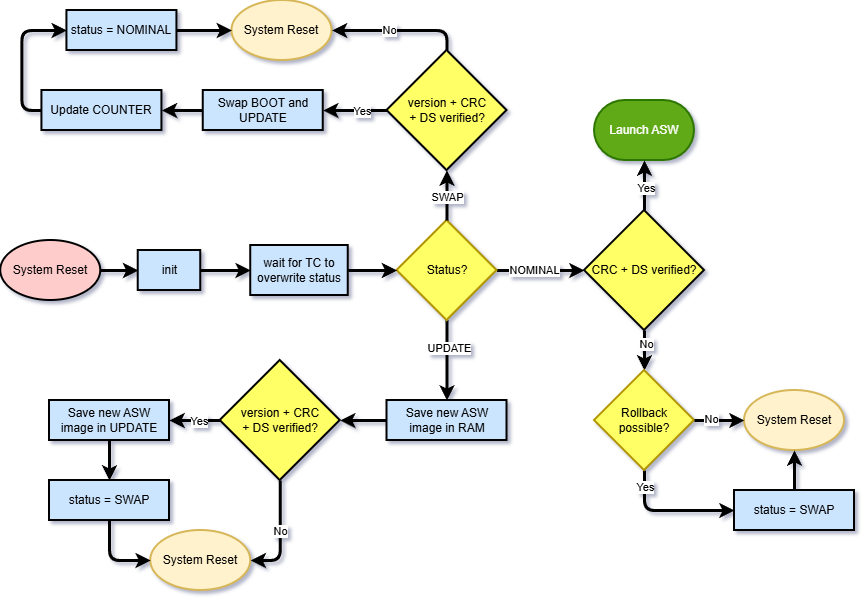
\includegraphics[width=0.8\linewidth]{figures/ESA Secure Boot Flowchart.Simple.png}
    \caption{Flowchart describing the boot process}
    \label{fig:bsw-flowchart}
\end{figure}

On every system reset, the hardware transfers execution directly to the BSW. After peripheral initialisation, the BSW opens a configurable reception window during which ground may send a command to select a specific mode. If no command arrives, the stored \texttt{COMM} status determines the mode entered. If a skip command is received, the stored status is used immediately without waiting for the full window to expire. A simplified flow diagram can be seen in \autoref{fig:bsw-flowchart}, while the overall detailed flow is captured in Figures \ref{fig:bsw-flowchart-startup}-\ref{fig:bsw-flowchart-rollback}.

\begin{figure}[h]
    \centering
    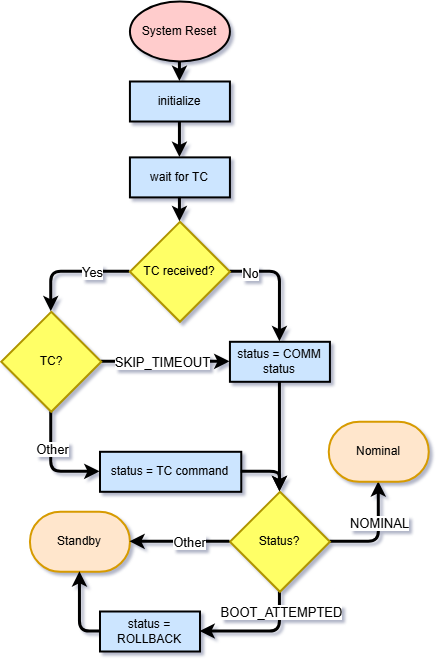
\includegraphics[width=0.4\linewidth]{figures/ESA Secure Boot Flowchart.Startup.png}
    \caption{Flowchart describing the startup process}
    \label{fig:bsw-flowchart-startup}
\end{figure}

At the start of each operation~--- nominal boot, firmware update or image swap~--- a new report record is created in RAM and its step-flag bitmask is updated incrementally as each phase completes. Writing flags to RAM rather than directly to flash avoids repeated small flash writes and reduces sector wear. At the end of the operation the finalised record is persisted to flash. Because flash must be erased at full sector granularity before new data can be written, all five existing report slots are first read into RAM, the REPORT sector is erased, and then the full buffer (including the new entry) is written back in a single operation. New reports are placed in the first empty slot if one exists. Once all five slots are occupied, the oldest entry is overwritten, implementing a circular buffer.

\subsection{State management}
\label{subsection:implementation-flow-state}

The BSW's persistent state is a single value written to the \texttt{COMM} partition. The  persistent states~--- \textsc{nominal}, \textsc{standby}, \textsc{swap},  \textsc{boot\_attempted}, \textsc{update}, \textsc{rollback}, and \textsc{report}~--- survive a system reset. Because the \texttt{COMM} partition is writeable by the ASW and therefore untrusted, the BSW never performs any image operations without first verifying their digital signatures. This ensures that the MAIN slot and \texttt{PROTECTED\_STATE} cannot be overwritten without a valid image in the UPDATE slot.

\subsection{Nominal mode flow}
\label{subsection:implementation-flow-nominal}

The nominal boot sequence enforces the following steps in order, as shown in \autoref{fig:bsw-flowchart-nominal}.

\begin{enumerate}
    \item \textbf{Protection check.}  The BSW verifies that the MAIN slot and \texttt{PROTECTED\_STATE} are write-protected.  If either is unprotected, it restores protection and resets before continuing, preventing an adversary who managed to disable protection from proceeding to image execution within the same boot cycle.

    \item \textbf{Boot-attempt stamp.}  The \texttt{COMM} status is set to \textsc{boot\_attempted} before any further action.  If the ASW subsequently crashes or resets without clearing this status, the next boot will detect the value and enter rollback evaluation rather than retrying the same failing image indefinitely.

    \item \textbf{CRC integrity check in flash.}  The hardware CRC32 of the image is computed and compared to the value stored in the image header.  A mismatch indicates flash corruption and triggers rollback without proceeding to the more expensive signature verification.

    \item \textbf{Copy to RAM.}  The full image is copied from the MAIN partition into RAM.

    \item \textbf{Signature verification.}  The signature field in the RAM copy is zeroed and digital signature verification is performed over the copied data.  A forged or corrupted image is rejected before execution.

    \item \textbf{CRC integrity check in RAM.}  The CRC check is repeated over the RAM copy to detect any corruption introduced during the copy operation.

    \item \textbf{Jump.}  The BSW disables all interrupts, clears the NVIC, deinitialises the HAL, sets the vector table offset register to the in-RAM image entry point and transfers execution to the application reset handler.
\end{enumerate}

The rationale for the ordering of these checks and their placement relative to the flash-to-RAM copy is discussed in \autoref{subsection:implementation-flow-sigseq}. \textsc{Boot\_attempted} is only cleared by the ASW itself, once it has determined that it is operating correctly, by updating the \texttt{COMM} partition.

\begin{figure}[h]
    \centering
    
\includegraphics[width=0.4\linewidth]{figures/ESA Secure Boot Flowchart.Nominal.png}
    \caption{Flowchart describing the nominal process}
    \label{fig:bsw-flowchart-nominal}
\end{figure}

\subsection{Standby mode - update and report}

In standby mode the BSW waits in a command loop, accepting one operation per received TC.
Ground can command a nominal boot, a firmware update, a swap of the current and pending images, a boot report, or a system reset.

\begin{figure}[h]
    \centering
    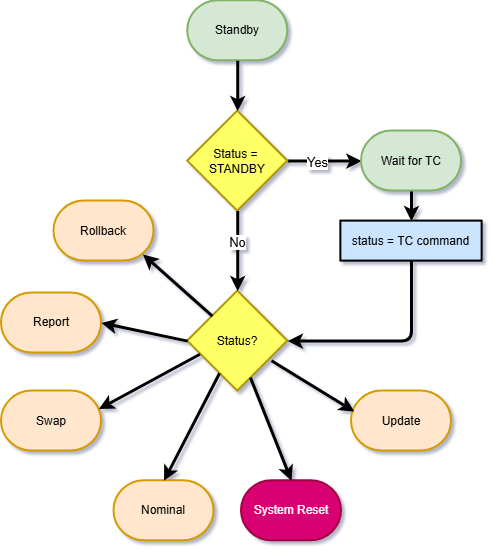
\includegraphics[width=0.4\linewidth]{figures/ESA Secure Boot Flowchart.Standby.png}
    \caption{Flowchart describing the standby process}
    \label{fig:bsw-flowchart-standby}
\end{figure}

A firmware update is received as a sequence of ECSS packets~--- a start packet carrying the total image size, a stream of data chunks and an end packet~--- and written to the UPDATE partition. A version and magic-number check on the first received chunk provides early rejection of obviously invalid images before the transfer completes. After all data has been received, a CRC check and digital signature verification are performed to prevent unnecessarily storing corrupt images. Once the data is written, the BSW configures for a swap and resets. Any error during the update process returns control to standby mode.

\begin{figure}[h]
    \centering
    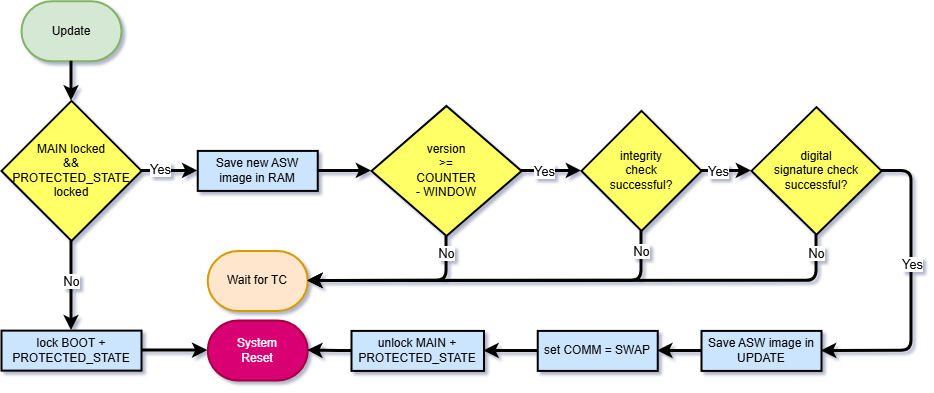
\includegraphics[width=0.7\linewidth]{figures/ESA Secure Boot Flowchart.Update.png}
    \caption{Flowchart describing the update process}
    \label{fig:bsw-flowchart-update}
\end{figure}

An image swap first validates the CRC, digital signature and version of the UPDATE slot before modifying the MAIN slot. Only after all three checks pass does the BSW execute the image exchange. Two mechanisms are supported and the choice between them reflects a trade-off relevant to space-grade hardware.

The \textbf{physical swap} performs a three-way copy (MAIN $\to$ SWAP, UPDATE $\to$ MAIN, SWAP $\to$ UPDATE), after which \texttt{SLOT\_A} always holds the active image and \texttt{SLOT\_B} always holds the previous image. This simplifies the nominal boot path: the BSW always loads from the same fixed flash address without consulting any index. The downside is that every update incurs three full sector erase--write cycles across \texttt{SLOT\_A}, \texttt{SLOT\_B} and \texttt{SWAP}. Radiation-tolerant flash memories used in space applications typically have a limited erase--write cycle budget, so this penalty is non-trivial over a long mission.

The \textbf{logical swap} instead updates only the primary slot index stored in \texttt{PROTECTED\_STATE}, making the UPDATE slot the new MAIN without copying any data. Because \texttt{PROTECTED\_STATE} is written on every swap regardless (to update the rollback counter), storing the index there adds no additional erase cycle. The three image sectors are left intact, extending their usable lifetime. The cost is a slightly more complex boot path: the BSW must read the index from \texttt{PROTECTED\_STATE} before it knows which address to load from.

In both cases the rollback counter is updated, write-protection is restored to reflect the new MAIN slot and the system resets. If any of the pre-swap checks fail, the BSW configures the system for nominal boot mode and restarts into standby mode.

\begin{figure}[h]
    \centering
    
\includegraphics[width=0.7\linewidth]{figures/ESA Secure Boot Flowchart.Swap.png}
    \caption{Flowchart describing the swap process}
    \label{fig:bsw-flowchart-swap}
\end{figure}

\subsection{Integrity and signature verification sequence}
\label{subsection:implementation-flow-sigseq}

The separation of CRC and signature verification, and their ordering relative to the flash-to-RAM copy, is intentional as it follows the SAVOIR requirements. The CRC is evaluated in flash first because it is cheap and detects silent flash corruption or uninitialised partitions before committing to a memory copy. The signature is evaluated only after the copy into RAM, as the digital signature field has to be modified, which would be impossible purely in flash. Zeroing the signature field before verifying and restoring it afterwards ensures that the byte sequence fed to the verification function is the same as what was used for signing the image in the first place. A secondary CRC check is performed before execution, to ensure that the transfer did not cause any memory corruption.


\section{Rollback protection implementation}
\label{section:implementation-rollback}

To satisfy \textbf{SEC.06}, three candidate designs for rollback protection were evaluated. All designs share one hard constraint: at least one partition must remain writable by the ASW to support autonomous in-orbit updates.

\subsection{Option A - version-based window, no counter}
\label{sub:rollback-a}

Under this scheme, there is no independent counter, but the rollback floor is derived directly from the version of the image currently in the MAIN partition, i.e.\ $v_{\min} = v_{MAIN} - X$. This design is vulnerable to an iterative downgrade attack. Consider a system running version~$N$ with window $X = 1$. The attacker uploads version $N-1$ to the UPDATE slot and triggers a rollback. Since $N-1 \geq N - 1$, the rollback is within the permitted window and is accepted. After the swap, MAIN now contains version~$N-1$. Because the floor is re-derived from the new MAIN version, it has also decreased to $N-2$. The attacker can therefore repeat the attack indefinitely, reducing the running version by one step per cycle until an arbitrarily old and vulnerable image is reached. Option~A was rejected for this reason.

\subsection{Option B - two partitions with monotonic counter}
\label{sub:rollback-b}

Option~B addresses the vulnerability in Option~A by storing the rollback floor in a separate, hardware-protected monotonic counter rather than deriving it from the mutable MAIN partition. The counter records the highest version that has ever been successfully executed and can only be incremented, never decremented, because it resides in a write-protected sector that only the BSW may modify. The rollback floor is $v_{\min} = N - X$, where $N$ is the counter value.

Under the same attack scenario, an attacker who triggers one permitted downgrade from version~$N$ to $N-1$ does not lower the counter, because the counter was set to~$N$ when version~$N$ was first executed. The floor therefore remains at $N-1$, and the next attempted downgrade to $N-2$ is rejected. The attack is thus bounded to a single step regardless of how many times the attacker controls the update channel. To perform a second downgrade, the attacker would first have to install and successfully execute a version higher than~$N$, which requires a valid signature from the private key.

\subsection{Option C - three partitions, no counter}
\label{sub:rollback-c}

A three-partition design can prevent iterative downgrade without a dedicated counter by separating the rollback and update code paths such that neither path can reach an arbitrarily old version through a sequence of individually valid operations. This option avoids the counter dependency at the cost of an additional flash partition and somewhat more complex swap logic.

In this scenario, both \texttt{SLOT\_A} and \texttt{SLOT\_B} are write-protected and a new \texttt{SLOT\_C} image partition is used to receive updates instead. To transfer an image to one of the main slots, its version and digital signature need to be verified, ensuring that an invalid image or an image version outside of the rollback window cannot be placed in \texttt{SLOT\_A} nor \texttt{SLOT\_B}. As the rollback operation swaps these protected partitions, the attack vector from Option A is no longer applicable even without a dedicated rollback counter.

\subsection{Selected approach and rationale}

While both Options A and B are a valid implementation, Option~B was selected as it provides strong, formally bounded rollback guarantees and is well-matched to the available hardware: the option-byte write protection of the STM32F439ZI makes implementing a dedicated counter sector straightforward.

The rollback window $X$ is set to~1, permitting recovery to the immediately preceding version while bounding any downgrade to a single step. This value is a compile-time constant defined in the BSW configuration. Missions requiring a different window size can adjust it at build time without modifying any other boot logic.
The rollback floor is defined as:
%
\begin{equation}
    v_{\min} = \max(0,\; N - X)
    \label{eq:rollback-floor}
\end{equation}
%
where $N$ is the monotonic counter value.
After any successful swap, the counter is updated to the maximum of
$N$, $v_{MAIN}$, and $v_{UPDATE}$, ensuring strict monotonicity. Before initiating a rollback, the BSW verifies two conditions: that the UPDATE version is strictly lower than the MAIN version (confirming the operation is a genuine downgrade) and that it satisfies \autoref{eq:rollback-floor}. Both conditions must hold simultaneously~--- failing either causes the BSW to enter the standby command loop and await ground intervention.

\begin{figure}
    \centering
    
\includegraphics[width=0.4\linewidth]{figures/ESA Secure Boot Flowchart.Rollback.png}
    \caption{Flowchart describing the rollback process}
    \label{fig:bsw-flowchart-rollback}
\end{figure}


\section{Cryptographic interface}
\label{section:implementation-crypto}

The cryptographic choices follow the algorithm recommendations discussed in \autoref{subsection:bg-space-cryptoReccs}. ECDSA-P256 and ML-DSA-65 are integrated into the PoC as the primary classical and post-quantum signature schemes, respectively. ECDSA was selected as the representative elliptic-curve-based signature scheme, while ML-DSA was selected as the representative lattice-based post-quantum signature scheme.

RSA-4096 and LMS are additionally included in the benchmarking campaign. RSA serves as a representative of traditional factorisation-based signatures, while LMS was selected as the representative hash-based post-quantum signature scheme. Compared to other hash-based schemes such as XMSS and SLH-DSA, LMS offers comparable security with favourable performance characteristics, making it a suitable candidate for resource-constrained environments \cite{wolfssl_lms_xmss_slhdsa}. Together, the selected algorithms represent the major families of digital signature schemes: factorisation-based (RSA), elliptic-curve-based (ECDSA), lattice-based (ML-DSA), and hash-based (LMS).

Key lengths are set in accordance with the recommendations discussed previously. The 4,096-byte signature field in the image header is sized to accommodate the largest expected signature (ML-DSA-65 at 3,309~bytes) alongside an ECDSA-P256 signature in hybrid mode, ensuring that the header format does not need to change when switching algorithm configurations.

\subsection{Algorithm-agnostic verification API}
\label{subsection:implementation-crypto-api}

The cryptographic module exposes a single \texttt{verifySignature()} function that accepts the signed byte buffer, its length and a pointer to the signature buffer. The calling code in the boot sequence is identical regardless of which algorithm is active. All algorithm selection is resolved at compile time through preprocessor defines.

The public keys are compiled as constant data directly into the BSW binary, placing them in the same write-protected flash sectors as the BSW code itself and satisfying \textbf{SEC.02} without any additional key storage mechanism. An alternative is to store only a hash of the public key in immutable memory and include the full key with each image upload; the BSW then hashes the received key and compares it against the stored hash before use, reducing the immutable storage requirement to 32--48~bytes regardless of algorithm. However, the full key must then be transmitted with every update and stored alongside each image in regular flash. For the PoC, which uses a single fixed key, storing the full key directly in write-protected flash is the simpler and equally secure choice.

All cryptographic primitives are provided by the wolfCrypt library rather than custom implementations, following the principle that cryptographic code should not be written from scratch without extensive validation. The \texttt{verifySignature()} function is also exposed through the BSP, so any subsequent software component~--- a stage-two bootloader or a dynamically loaded module~--- can verify further components using the same root of trust without duplicating cryptographic logic.

\subsection{Classical algorithms - ECDSA}
The classical implementation uses ECDSA-P256 with the wolfCrypt library, in compliance with the recommendations discussed in \autoref{subsection:bg-space-cryptoReccs}. The public key is stored in standard DER SubjectPublicKeyInfo encoding. SHA-256 is computed over the signed buffer region and the resulting digest is passed to the signature verification function. The DER encoding carries the signature length explicitly, so signatures of varying length can be handled correctly without knowing the signature in advance.

\subsection{Post-quantum algorithms - ML-DSA}

The post-quantum implementation uses ML-DSA-65 (NIST FIPS~204~\cite{nist_ml_dsa}, security level~3), also via wolfCrypt. Unlike ECDSA, ML-DSA operates directly on the full message and performs its own internal hashing, so no pre-computation of a digest is required.

\subsection{Hybrid algorithms - ECDSA + ML-DSA}

In hybrid mode, both algorithms must succeed for the image to be accepted, as recommended during the post-quantum transition period~\cite{bsi_crypto_key_length}. The 4\,096-byte signature field is partitioned so that the ECDSA signature occupies the first 72~bytes (the maximum DER-encoded length for P-256) and the ML-DSA signature occupies the following 3\,309~bytes, for a combined total of 3\,381~bytes. ECDSA verification is performed first; if either verification fails, the image is rejected immediately.

The algorithm-agnostic API, compile-time algorithm selection and wolfCrypt-backed primitives together ensure that switching between classical, post-quantum and hybrid deployments requires only a build-flag change, with no modifications to the boot sequence logic or the image format. This directly satisfies \textbf{SEC.05} and leaves the door open for adopting future NIST-standardised algorithms as they become available in the library.